% COntinued Chpater Implementation
\section{Content Based Model}

The content-based model uses vector space models of a user and an item to find the similarity between two vectors. The overview of content-based model is discussed in the \autoref{fig:content_based_flowchart}. 

\begin{figure}[H]
	\centering
	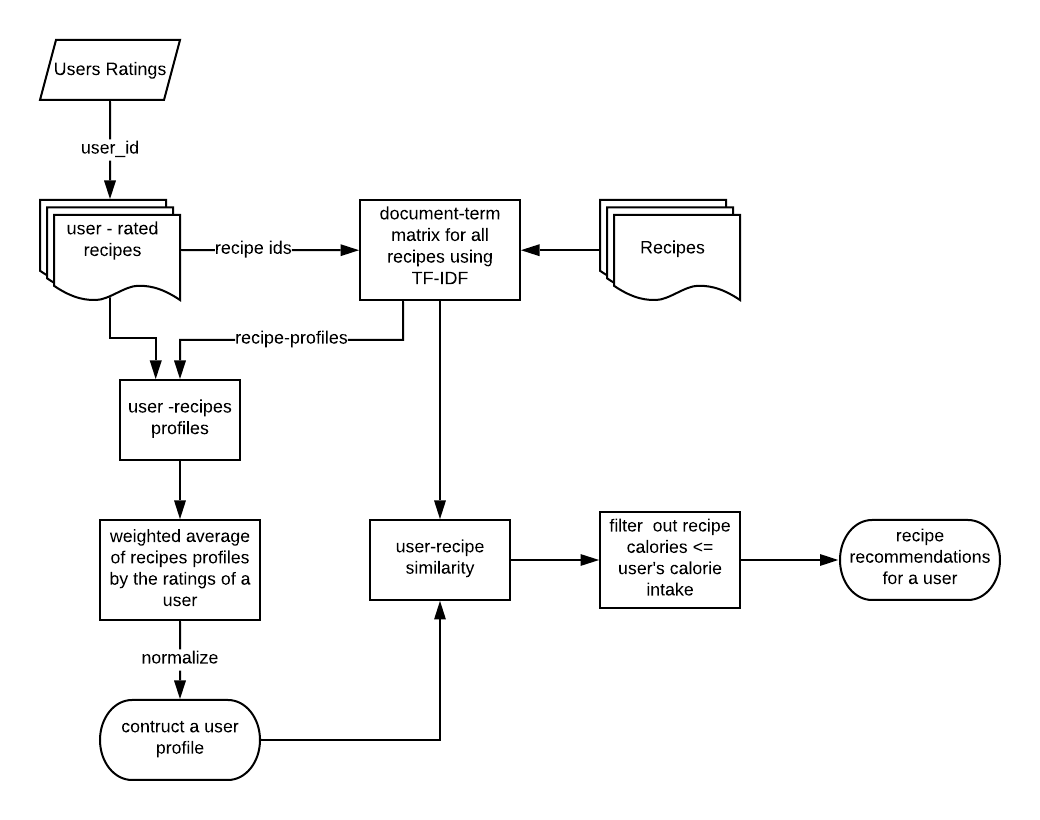
\includegraphics[width=1.0\linewidth]{content_based_flowchart}
	\caption{Content Based Filtering Work-Flow }
	\label{fig:content_based_flowchart}
\end{figure}  

\noindent
All user interactions are denoted by 'Users Ratings' and all recipes information is denoted by 'Recipes'. Required steps to generated a user profile and a recipe profile are discussed below.
\begin{itemize}
\item All recipe profiles are generated based on the relevancy of terms to be considered. The term may vary based on the application area. In this thesis, ingredients, cooking methods, and diet labels are considered. The relevancy of terms in the documents is measured by TF-IDF as discussed in \nameref{sec:tf-idf}. A document term matrix is generated and stored for all recipes. 
\item Rated recipes for a single user are filtered from all user interactions.
Rated recipes are then filtered out and stored from a stored document-term matrix. 
\item To construct a user profile, recipes vectors rated by a user are considered. Then a weighted average of rated recipe profiles is calculated. The user profile is further normalized on the weighted values. 
\item Similarity between the user profile and all recipe profiles from the dataset is measured by cosine similarity as discussed in \nameref{cosine_similarity}. Recipes that are rated previously by the user are omitted to calculate relevance. Sort these recipes in descending order of similarity scores.
\item On the resultant recipes vectors we have applied a calorie intake filter comparing recipe calories and user required calories. These recipes are offered as recommendations to the user.  
\end{itemize}
 

\subsection{Content-Based Using Ingredients}
Recipe ingredients are used to calculate recommendations in content-based using ingredients approach. The user profile and recipe profiles are generated using ingredients in the recipes. The steps to generate recommendations for a user using ingredients in content based model are discussed below.
\begin{itemize}
\item All ingredients from recipes are extracted. 
\item Similarity between recipes are considered based on ingredients but there are many ingredients are commonly used in all recipes such as salt. To get the importance of ingredients which are relevant to the recipe and to negate effect of high frequency terms, concept of TF-IDF has been used as discussed in \nameref{sec:tf-idf}. The recipe vector or recipe profile is calculated for each recipe in the dataset. The 'TfidfVectorizer' function from 'sklearn' has been used to calculate TF-IDF.
\item The weighted average of a user rated recipe profiles is calculated to construct a user profile. Constructed user profile is based on ingredients of the recipes.  
\item Similarity between a user profile and all recipe profiles in the dataset is calculated using cosine similarity. The 'linear\_kernel' function from the 'sci-kit learn' library has been used for the same. 
\item The resultant profiles are listed in descending order of similarity score to get more relevant recipes at top. At this point recipes already rated by a user are omitted. 
\item From user's information, the BMR and the required calorie intake per meal is calculated. 
\item The resultant set of recipes are offered as recommendations. 
\end{itemize}
\subsubsection{Experiment}
\label{sec:cb_ingred_exp}

\subsection{Recommendations Using Ingredients and Cooking Methods}
\subsubsection{Experiment}
\label{sec:cb_ingred_cook_method_exp}
\subsection{Recommendations Using Ingredients, Cooking Method and Diet Labels}
\subsubsection{Experiment}
\label{sec:cb_ingred_cook_method_diet_label_exp}

\section{Collaborative Filtering Model}
Model-based collaborative filtering for the user and recipes was applied. This approach utilizes information related to user ratings on the recipes. A Singular Value Decomposition algorithm has been applied to get the recommendations. The below approach was followed to get recommendations using SVD.

\begin{figure}[H]
	\centering
	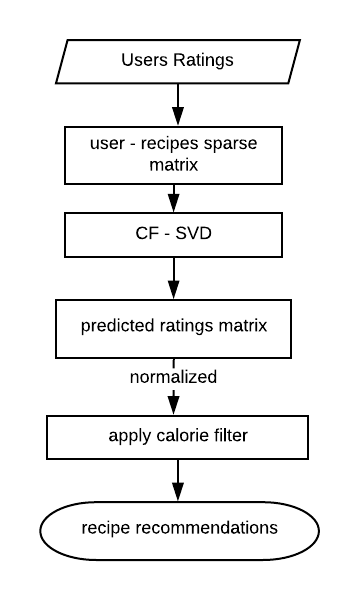
\includegraphics[width=0.5 \linewidth]{cf-svd}
	\caption{Collaborative Filtering- SVD Work-Flow }
	\label{fig:cf-svd}
\end{figure}  

\begin{itemize}
\item All user ids and recipe ids are extracted in such a way that every user id and recipe id represents a unique relationship via rating. The user id refers to unique id given to the user and recipe id refers to a unique id given to the recipe in the dataset. The matrix of user-recipes ratings is formed such as a user represents row and recipes represents columns. The cell value represents a rating for a recipe given by a user. From this matrix, the sparse matrix was created. 
\item The sparse matrix is the same as above matrix except it has high efficiency to perform large mathematical operations. To create a sparse matrix, 'csr\_matrix' function is used from 'scipy.sparse' library. The generated sparse matrix was sent as an input to the SVD algorithm.
\item SVD algorithm runs PCA on the user-rating matrix to give back factors of the rating matrix as discussed in \nameref{sec:svd}. The dot product of these factors returns a rating matrix with predicted ratings. 
\item Further, normalization was performed to get all predicted ratings for all users for all recipes.
\end{itemize}

\subsection{Experiment}
\label{sec:svd_exp}
\section{Hybrid Filtering Model(CB and CF)}
